%!TEX root = supplement.tex

%%%%%%%%%%%%%%%%%%%
\begin{figure}
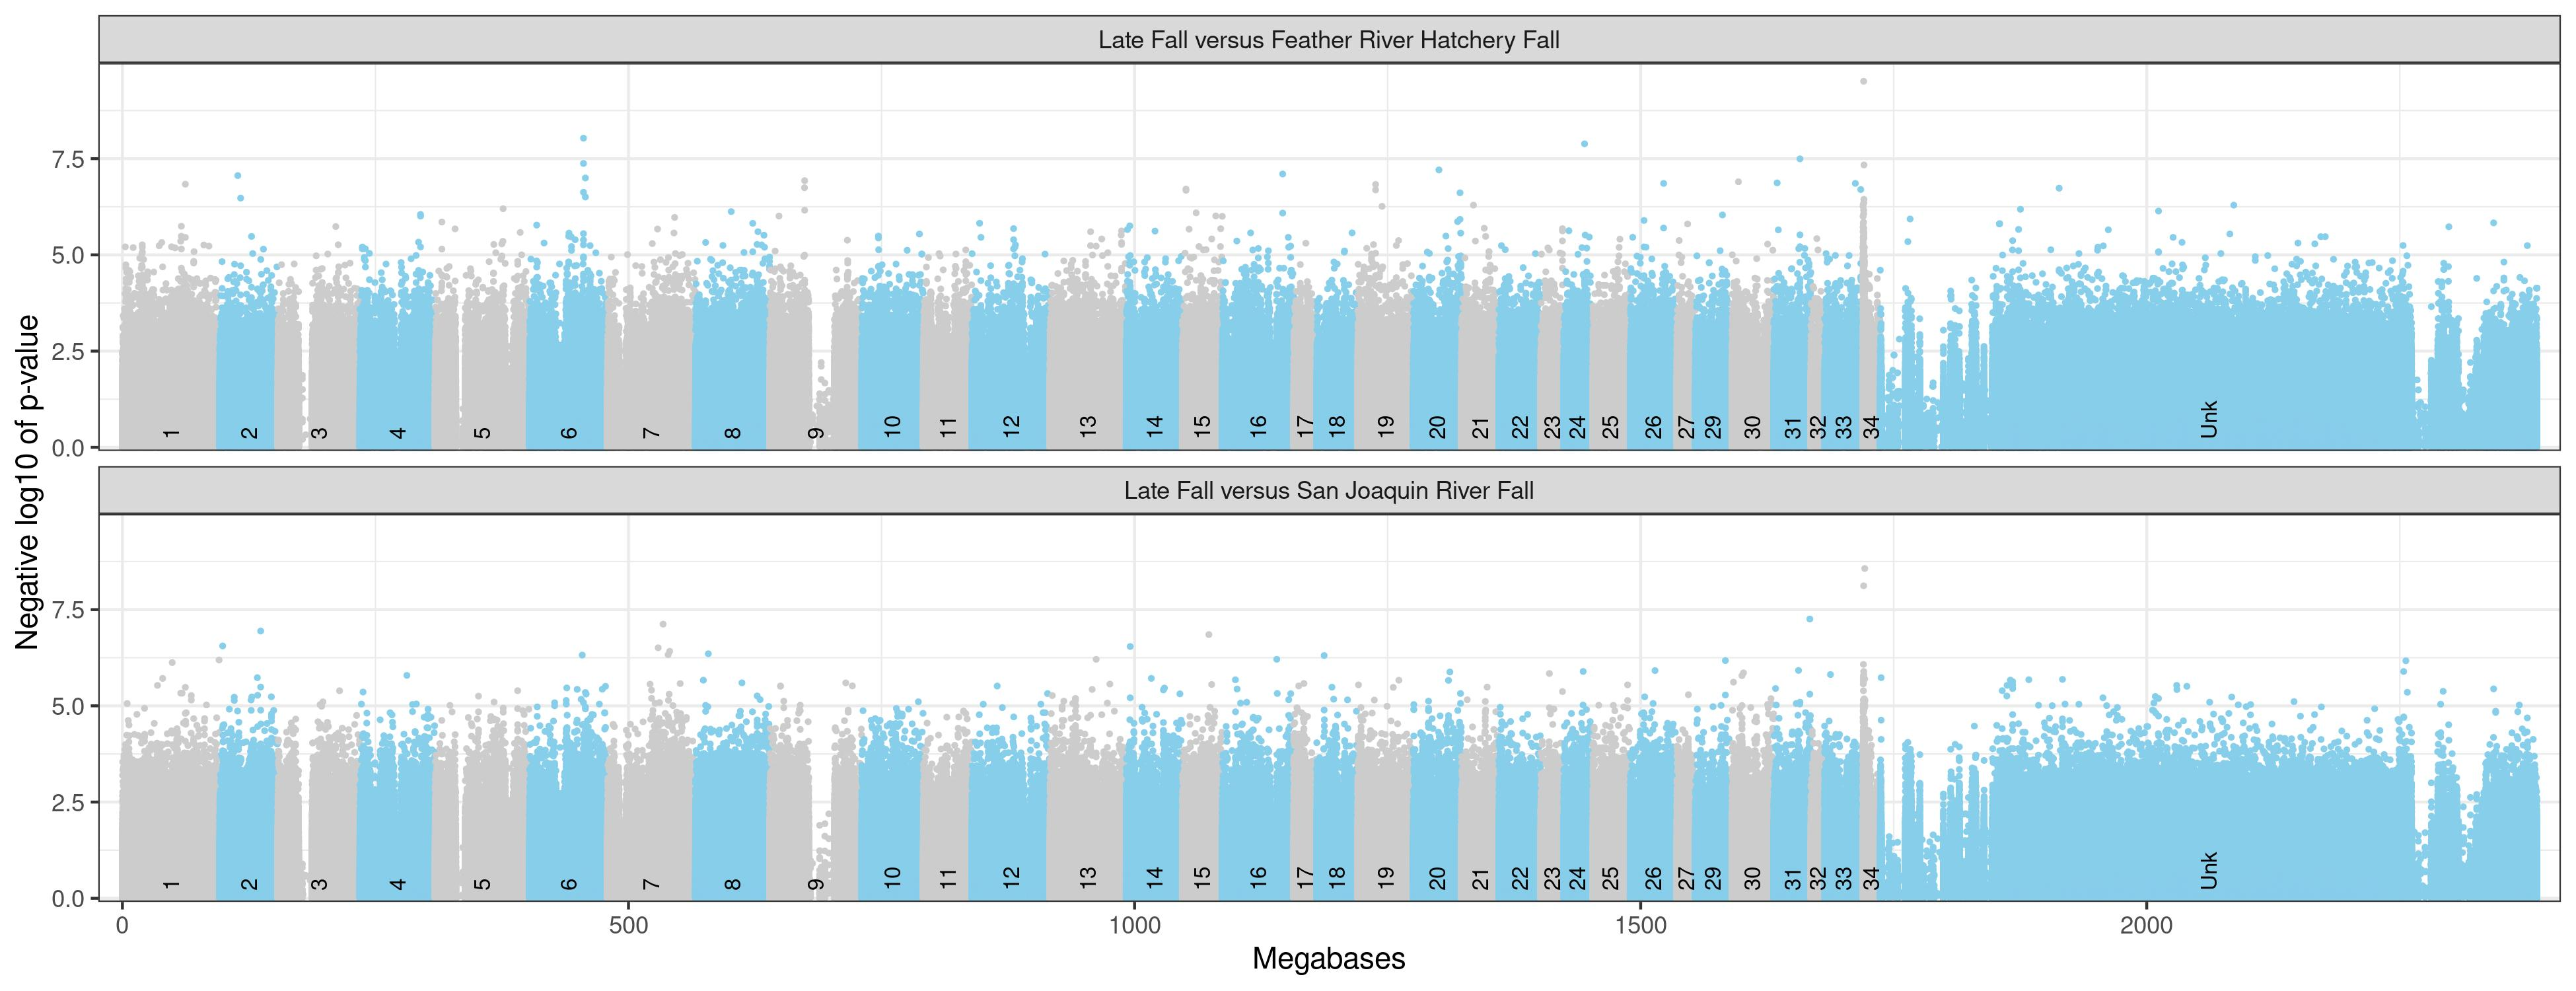
\includegraphics[width=\textwidth]{images/lfar-assoc-faceted.jpg}
\caption[
	Negative log base 10 of association $p$-values for
	individual SNPs for late-fall versus fall run
]{
	\footnotesize Negative log base 10 of association $p$-values for
	individual SNPs for late-fall versus fall run.  $x$ axis shows position in genome (in megabases),
	with color alternating by chromosome, as indicated by numbers above the $x$-axis. ``Unk'' refers
	to unplaced scaffolds in the Otsh\_v1.0 genome assembly \citep{christensen2018chinook}. The 
	upper panel is the comparison between late-fall and Feather River Hatchery fall, while the lower 
	panel is the comparison of late-fall to San Joaquin River fall. 
}
\label{fig:lfar-assoc}
\end{figure}



%%%%%%%%%%%%%%%%%%%%%% 
\begin{figure}
\begin{center}
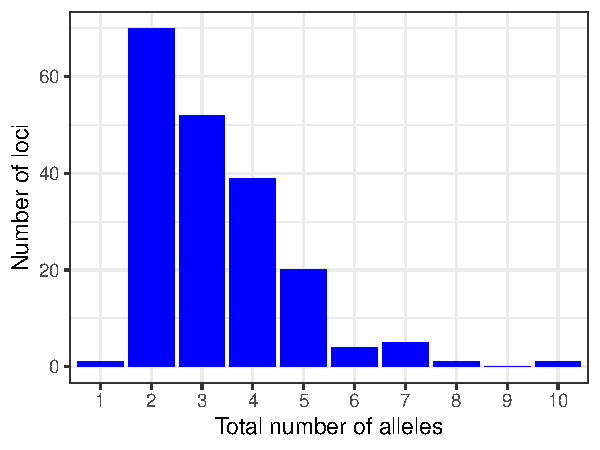
\includegraphics[width=0.7\textwidth]{images/num-alle-barplot.pdf}
\end{center}
\caption[Number of loci with different
total numbers of alleles]{\footnotesize Number of loci with different
total numbers of alleles in the data set.}
\label{fig:num-alle}
\end{figure}
%%%%%%%%%%%%%%%%%%%%

